%\documentclass[12pt]{article}
\documentclass[14pt,a4paper]{extarticle}
%%---------------------------------------------------------------------
% packages
% geometry
\usepackage{geometry}
% font
\usepackage{xeCJK}
\xeCJKsetup{CJKmath=true,CheckSingle=true}
\usepackage{pifont}  % \ding{}
% math
\usepackage{amsmath,amsfonts,amssymb}
% color
\usepackage{color}
\usepackage{xcolor}
\definecolor{EYE}{RGB}{199,237,204}
\definecolor{FLY}{RGB}{128,0,128}
\definecolor{ZHY}{RGB}{139,0,255}
\definecolor{bgcode}{rgb}{0.95,0.95,0.95}
% graphics
\usepackage[americaninductors,europeanresistors]{circuitikz}
\usepackage{tikz}
\usetikzlibrary{positioning,arrows,shadows,shapes,calc,mindmap,trees,backgrounds}  % placements=positioning
\usepackage{graphicx}  % \includegraphics[]{}
\usepackage{subfigure}  %%图形或表格并排排列
% table
\usepackage{colortbl,dcolumn}  %% 彩色表格
\usepackage{multirow}
\usepackage{multicol}
\usepackage{booktabs}
% code
\usepackage{fancyvrb}
\usepackage{listings}
\usepackage{minted}
% title
\usepackage{titlesec}
% head/foot
\usepackage{fancyhdr}
% ref
\usepackage{hyperref}
% pagecolor
\usepackage[pagecolor={EYE}]{pagecolor}
% tightly-packed lists
\usepackage{mdwlist}
% Waldi Symbol
\usepackage{wasysym} % \smiley
% cvbiouc-defined
\usepackage{styles/iplouccfg}
%\usepackage{styles/zhfontcfg}
\usepackage{styles/iplouclistings}

%%---------------------------------------------------------------------
% settings
% geometry
\geometry{left=2cm,right=1cm,top=2cm,bottom=2cm}  %设置 上、左、下、右 页边距
\linespread{1.5} %行间距
% font
\setCJKmainfont[AutoFakeBold,AutoFakeSlant]{Adobe Kaiti Std} %默认字体:楷体
\setCJKmonofont{Adobe FangSong Std} %设置\ttfamily字体
%\setmainfont[BoldFont=Adobe Garamond Pro Bold]{Apple Garamond}  % 英文字体
%\setmainfont[BoldFont=Adobe Garamond Pro Bold,SmallCapsFont=Apple Garamond,SmallCapsFeatures={Scale=0.7}]{Apple Garamond}  %%苹果字体没有SmallCaps
% graphics
\graphicspath{{figures/}}
\tikzset{
    % Define standard arrow tip
    >=stealth',
    % Define style for boxes
    punkt/.style={
           rectangle,
           rounded corners,
           draw=black, very thick,
           text width=6.5em,
           minimum height=2em,
           text centered},
    % Define arrow style
    pil/.style={
           ->,
           thick,
           shorten <=2pt,
           shorten >=2pt,},
    % Define style for FlyZhyBall
    FlyZhyBall/.style={
      circle,
      minimum size=6mm,
      inner sep=0.5pt,
      ball color=red!50!blue,
      text=white,},
    % Define style for FlyZhyRectangle
    FlyZhyRectangle/.style={
      rectangle,
      rounded corners,
      minimum size=6mm,
      ball color=red!50!blue,
      text=white,},
    % Define style for zhyfly
    zhyfly/.style={
      rectangle,
      rounded corners,
      minimum size=6mm,
      ball color=red!25!blue,
      text=white,},
    % Define style for new rectangle
    nrectangle/.style={
      rectangle,
      draw=#1!50,
      fill=#1!20,
      minimum size=5mm,
      inner sep=0.1pt,}
}
\ctikzset{
  bipoles/length=.8cm
}
\newcommand\zhyfly[1]{\vspace{.2em}\tikz \node[rectangle,rounded corners,minimum size=6mm,ball color=FLY,text=white,]{#1};\vspace{-.2em}}
% code
\renewcommand{\theFancyVerbLine}{\sffamily\textcolor[rgb]{0.5,0.5,1.0}{\scriptsize\oldstylenums{\arabic{FancyVerbLine}}}}
\newminted{c}{breaklines,linenos,numbersep=5pt,mathescape,bgcolor=bgcode}
\newminted{cpp}{breaklines,linenos,numbersep=5pt,mathescape,bgcolor=bgcode}
\newminted{bash}{breaklines,linenos,numbersep=5pt,mathescape,bgcolor=bgcode}
%% \begin{frame}[fragile=singleslide]
%% \begin{ccode}
%% //http://www.roesler-ac.de/wolfram/hello.htm
%% /* Hello World in C, Ansi-style */
%% 
%% #include <stdio.h>
%% #include <stdlib.h>
%% 
%% int main(void)
%% {
%%   puts("Hello World!");
%%   return EXIT_SUCCESS;
%% }
%% \end{ccode}
%% \mint{c}|print(("Hello World!");|
%% \end{frame}
\lstnewenvironment{clstcode}[1][]{%
  \lstset{
    basicstyle=\footnotesize\ttfamily\color{black},%
    columns=flexible,%
    framexleftmargin=.7mm,frame=shadowbox,%
    rulesepcolor=\color{blue},%
%    frame=single,%
    backgroundcolor=\color{yellow!20},%
    keywordstyle=\bf\color{blue},%
    identifierstyle=\bf,%
    commentstyle=\it\color[RGB]{0,96,96},%
    stringstyle=\rmfamily\slshape\color[RGB]{128,0,0},%
    showstringspaces=false,%
    xleftmargin=1.2\fboxsep,%
    xrightmargin=.7\fboxsep,%
    numbers=left,numberstyle=\tiny\color{blue},%
    numberblanklines=false,numbersep=7pt,%
    language=[ANSI]C%
    }\lstset{#1}}{}
\lstnewenvironment{clstmiddle}[1][]{%
  \lstset{
    basicstyle=\scriptsize\ttfamily\color{black},%
    columns=flexible,%
    framexleftmargin=.7mm,frame=shadowbox,%
    rulesepcolor=\color{blue},%
%    frame=single,%
    backgroundcolor=\color{yellow!20},%
    backgroundcolor=\color{yellow!20},%
    keywordstyle=\bf\color{blue},%
    identifierstyle=\bf,%
    commentstyle=\it\color[RGB]{0,96,96},%
    stringstyle=\rmfamily\slshape\color[RGB]{128,0,0},%
    showstringspaces=false,%
    xleftmargin=1.2\fboxsep,%
    xrightmargin=.7\fboxsep,%
    numbers=left,numberstyle=\tiny\color{blue},%
    numberblanklines=false,numbersep=7pt,%
    language=[ANSI]C%
    }\lstset{#1}}{}
\lstnewenvironment{clstsmall}[1][]{%
  \lstset{
    basicstyle=\tiny\ttfamily\color{black},%
    columns=flexible,%
    framexleftmargin=.7mm,frame=shadowbox,%
    rulesepcolor=\color{blue},%
%    frame=single,%
    backgroundcolor=\color{yellow!20},%
    backgroundcolor=\color{yellow!20},%
    keywordstyle=\bf\color{blue},%
    identifierstyle=\bf,%
    commentstyle=\it\color[RGB]{0,96,96},%
    stringstyle=\rmfamily\slshape\color[RGB]{128,0,0},%
    showstringspaces=false,%
    xleftmargin=1.2\fboxsep,%
    xrightmargin=.7\fboxsep,%
    numbers=left,numberstyle=\tiny\color{blue},%
    numberblanklines=false,numbersep=7pt,%
    language=[ANSI]C%
    }\lstset{#1}}{}
% pdf
\hypersetup{pdfpagemode=FullScreen,%
            pdfauthor={Haiyong Zheng},%
            pdftitle={Title},%
            CJKbookmarks=true,%
            bookmarksnumbered=true,%
            bookmarksopen=false,%
            plainpages=false,%
            colorlinks=true,%
            citecolor=green,%
            filecolor=magenta,%
            linkcolor=cyan,%red(default)
            urlcolor=cyan}
% section
%http://tex.stackexchange.com/questions/34288/how-to-place-a-shaded-box-around-a-section-label-and-name
\newcommand\titlebar{%
\tikz[baseline,trim left=3.1cm,trim right=3cm] {
    \fill [cyan!25] (2.5cm,-1ex) rectangle (\textwidth+3.1cm,2.5ex);
    \node [
        fill=cyan!60!white,
        anchor= base east,
        rounded rectangle,
        minimum height=3.5ex] at (3cm,0) {
        \textbf{\thesection.}
    };
}%
}
\titleformat{\section}{\Large\bf\color{blue}}{\titlebar}{0.1cm}{}
% head/foot
\setlength{\headheight}{15pt}
\pagestyle{fancy}
\fancyhf{}
\lhead{\color{black!50!green}2017年}
\chead{\color{black!50!green}VISION@OUC第一阶段}
\rhead{\color{black!50!green}中国海洋大学}
\lfoot{\color{blue!50!green}郑海永/俞智斌/王楠}
\cfoot{\color{blue!50!green}\href{http://vision.ouc.edu.cn}{VISION@OUC}}
\rfoot{\color{blue!50!green}$\cdot$\ \thepage\ $\cdot$}
\renewcommand{\headrulewidth}{0.4pt}
\renewcommand{\footrulewidth}{0.4pt}

%%---------------------------------------------------------------------
\begin{document}
%%---------------------------------------------------------------------
%%---------------------------------------------------------------------
% \titlepage
\title{\vspace{-2em}VISION@OUC第一阶段任务(入学前)\vspace{-0.7em}}
\author{郑海永 俞智斌 王楠}
\date{\vspace{-0.7em}2016年\vspace{-0.7em}}
%%---------------------------------------------------------------------
\maketitle\thispagestyle{fancy}
%%---------------------------------------------------------------------
\maketitle
\tableofcontents

\section{基础能力}

\subsection{技术}

\begin{description}
\item[操作系统] GNU/Linux,推荐Ubuntu。
\item[\textcolor{red}{编程语言}] C/C++和Python,此项非常重要!

关于程序设计,推荐北京大学专项课程“\href{https://www.coursera.org/specializations/biancheng-suanfa}{程序设计与算法}”(\href{http://vision.ouc.edu.cn/~zhenghaiyong/courses/oop/2017spring/mooc/}{资源下载})
\item[代码管理] GitHub
\item[文档排版] \LaTeX{}
\end{description}

\subsection{专业}

\begin{description}
\item[数字图像处理] 建议:Digital Image Processing (3rd edition), by Rafael Gonzalez and Richard Woods, Prentice Hall, 2008.
\item[计算机视觉] 建议:Computer Vision: Algorithms and Applications, by Richard Szeliski, Springer, 2010.
\item[机器学习] 建议:《机器学习》,周志华,清华大学出版社,2016年。
\end{description}

\subsection{要求}

\begin{enumerate}
\item 每人创建GitHub帐号进行学习过程中的代码和文档(包括笔记等)管理。
\item 所有的笔记等文档全部使用\LaTeX{}来撰写。
\item 所有的专业知识学习要求必须有对应的代码和实验及记录等文档。
\end{enumerate}

\subsection{考核}

\begin{enumerate}
\item \textbf{GitHub}:入学时我们会详细查阅每个人的GitHub中的代码和文档等来评估是否对学习过程进行了详细的记录和整理,尤其自己的思考和问题等。
\item \textbf{答辩}:入学后一周内进行现场答辩,将自己对上述所学及下述感兴趣研究方向的方方面面进行汇报,并接受老师质疑,时间每人不超过1小时。
\end{enumerate}

\section{研究方向}

\subsection{郑海永}

主要的研究方向为\textbf{图像识别}或\textbf{图像分类},在此问题下又分为以下两个方面:
\begin{enumerate}
\item \textbf{中文}:细粒度图像分类/图像精细识别

\textbf{English}: Fine-Grained Visual Classification / Fine-Grained Image Classificaion / Fine-Grained Image Recognition

\textbf{简要说明}:通过图像识别是狗还是鸟相对比较容易,而如果从鸟中识别是哪一种鸟(生物分类阶元:界门纲目科属种),则难上加难(可能只有生物分类专家才能做到),如图\ref{fig:FGIR}所示。

\textbf{主要方法}:深度神经网络(Deep Neural Network)
\begin{figure}[!ht]
  \centering
  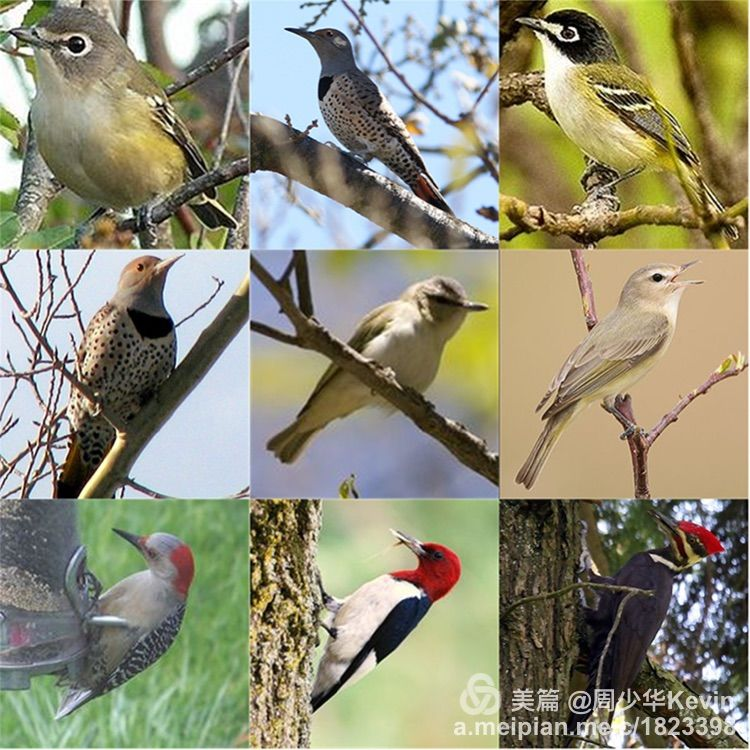
\includegraphics[width=0.8\textwidth]{FGIR.jpg}
  \caption{图像精细识别}
  \label{fig:FGIR} %% label for entire figure
\end{figure}
\item \textbf{中文}:不平衡数据(图像)分类

\textbf{English}: Imbalanced Data (Image) Classification

\textbf{简要说明}:类别不平衡现象广泛存在于现实生活中的大量实际应用中,比如你看到“老虎”的样本数要远少于你看到“狗”的样本数,那么对于多数类样本和少数类样本的分类问题,就很难用传统的机器学习方法来解决。例如,假设一个数据集包括2类,其中多数类样本数为99、少数类样本数为1,那么分类器可以直接忽视掉少数类(全部样本识别为多数类)便可以得到99\%的识别准确率,尽管这个识别准确率已经算很高了,但是对于少数类的识别准确率却为0,而有时候少数类的识别准确率可能更重要,比如诊断癌症、信用诈骗等。

\textbf{主要方法}:类别不平衡学习(Class-Imbalance Learning)、生成式对抗网络(Generative Adversarial Network)
\item \textbf{中文}:图像质量评价

\textbf{English}: Image Quality Assessment (IQA)

\textbf{简要说明}:图像质量评价是图像处理中的基本技术之一,主要通过对图像进行特性分析研究,然后评估出图像优劣(图像失真程度)。图像质量评价在图像处理系统中,对于算法分析比较、系统性能评估等方面有着重要的作用。近年来,随着对数字图像领域的广泛研究,图像质量评价的研究也越来越受到研究者的关注,提出并完善了许多图像质量评价的指标和方法。

\textbf{主要方法}:主观评价和客观评价,客观评价包括全参考(Full-Reference,FR)、部分参考(Reduced-Reference,RR)和无参考(No-Reference,NR)三种类型。
\end{enumerate}

\subsection{俞智斌}

%基于双目的水下深度图像估计、不同光场下的水质参数反演以及基于神经网络的水下图像复原
%基于双目的深度图像估计、基于图像的参数回归以及基于退化模型的图像复原
\begin{enumerate}
\item \textbf{中文}:深度图像估计/图像深度估计。

\textbf{English}: Depth Map Prediction / Depth Map Estimation / Depth Prediction / Depth Estimation.

\textbf{简要说明}:通过一副或多幅图像预测/估计图像中每个物体(像素)的深度信息。如图\ref{fig:depth}所示,图\ref{fig:depth:a}表示原始图像,图\ref{fig:depth:b}为真实的深度图(可以通过微软Kinect等设备采集获得),图\ref{fig:depth:c}为通过所研究的方法(算法)由图\ref{fig:depth:a}所得到的预测深度图。实际应用时,我们只通过原始图像就可以计算得到(预测)深度图,那么方法(算法)的好坏就由预测/估计的准确性来评判。

\textbf{主要方法}:深度神经网络(Deep Neural Network)
\begin{figure}[!ht]
  \centering
  \subfigure[原图]{
    \label{fig:depth:a} %% label for first subfigure
    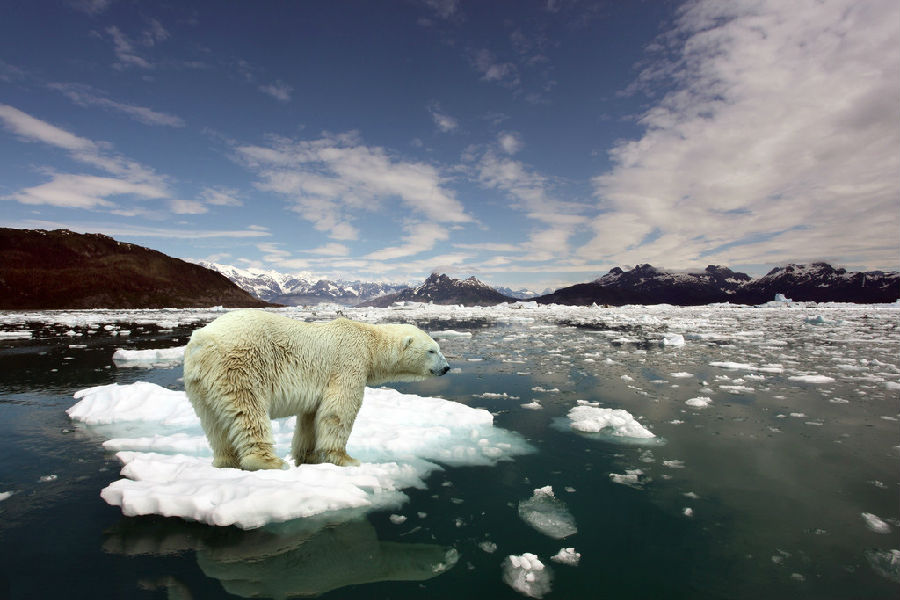
\includegraphics[width=0.3\textwidth]{DepthOrig.jpg}}
%  \hspace{1em}
  \subfigure[真实深度图]{
    \label{fig:depth:b} %% label for second subfigure
    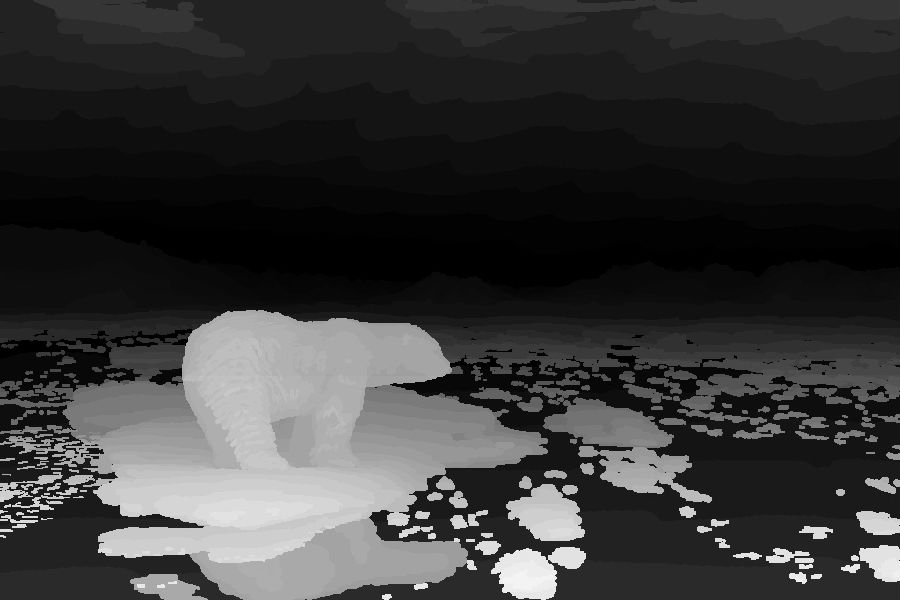
\includegraphics[width=0.3\textwidth]{DepthTruth.jpg}}
%  \hspace{1em}
  \subfigure[预测深度图]{
    \label{fig:depth:c} %% label for second subfigure
    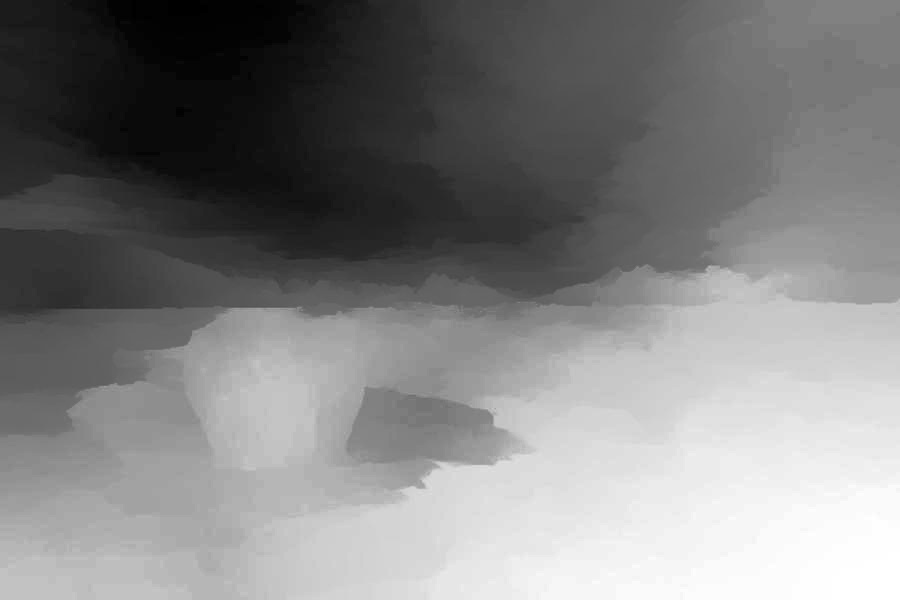
\includegraphics[width=0.3\textwidth]{DepthPrediction.jpg}}
  \caption{深度图像估计/图像深度估计}
  \label{fig:depth} %% label for entire figure
\end{figure}

\item \textbf{中文}:图像复原。

\textbf{English}: Image Restoration.

\textbf{简要说明}:图像复原就是利用退化过程的先验知识,去恢复已被退化图像的本来面目。成像系统受各种因素的影响,导致了图像质量的降低,称之为图像退化。因素包括:传感器噪声、摄像机聚焦不佳、物体与摄像机之间的相对移动、随机大气湍流、光学系统的象差、成像光源和射线的散射等。 退化基本表现:图像模糊。如图\ref{fig:dehaze}所示为北京灰霾的照片及其去雾结果,图\ref{fig:deblur}所示为模糊图像及其去模糊结果和去模糊所用到的模糊核。图像去雾(dehaze)和图像去模糊(deblur)可以应用图像复原方法来处理。
\begin{figure}[!ht]
  \centering
  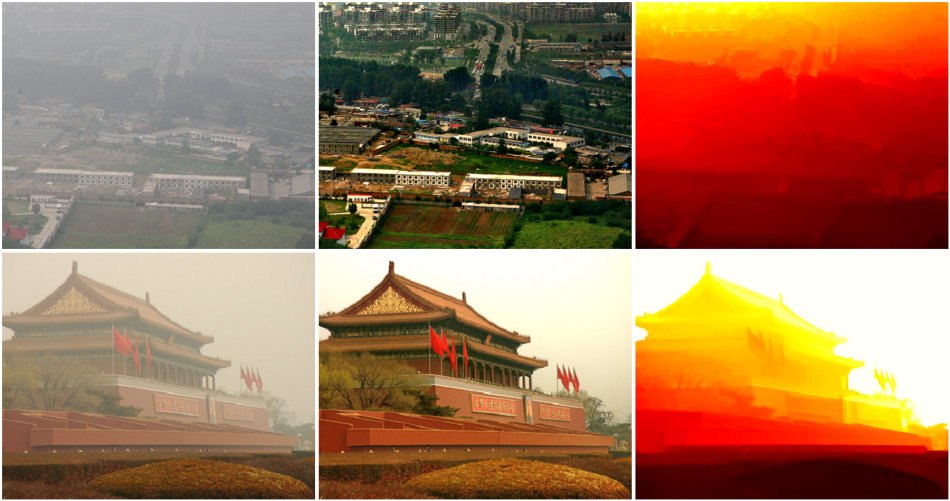
\includegraphics[width=0.9\textwidth]{Dehaze.jpg}
  \caption{图像去雾(Dehaze)}
  \label{fig:dehaze} %% label for entire figure
\end{figure}
\begin{figure}[!ht]
  \centering 
  \subfigure[原图]{ 
    \label{fig:deblur:a} %% label for first subfigure
    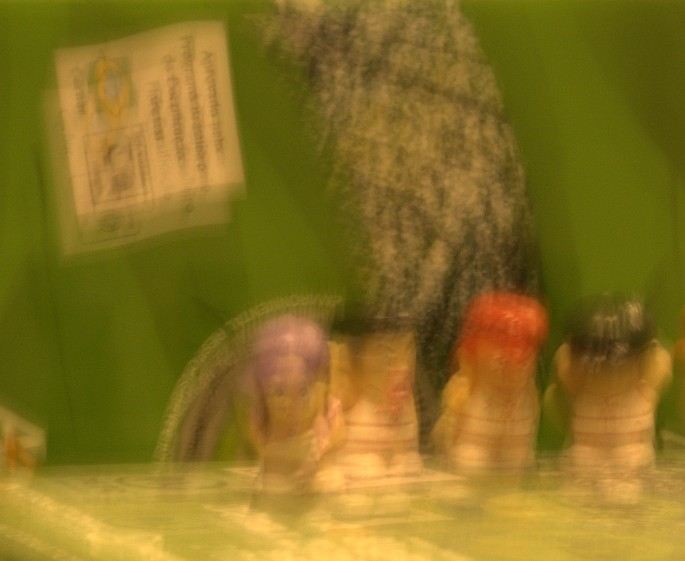
\includegraphics[width=0.4\textwidth]{DeblurOrig.jpg}}
%  \hspace{1em}
  \subfigure[去模糊图像]{
    \label{fig:deblur:b} %% label for second subfigure
    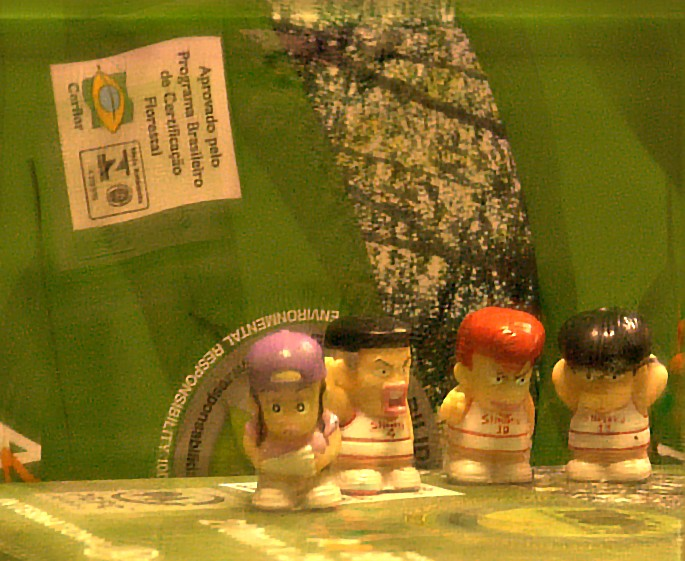
\includegraphics[width=0.4\textwidth]{DeblurResult.jpg}}
%  \hspace{1em}
  \subfigure[模糊核]{
    \label{fig:deblur:c} %% label for second subfigure
    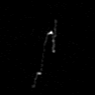
\includegraphics[width=0.15\textwidth]{DeblurKernel.png}}
%  \\
%  \subfigure[原图]{
%    \label{fig:deblur:d} %% label for first subfigure
%    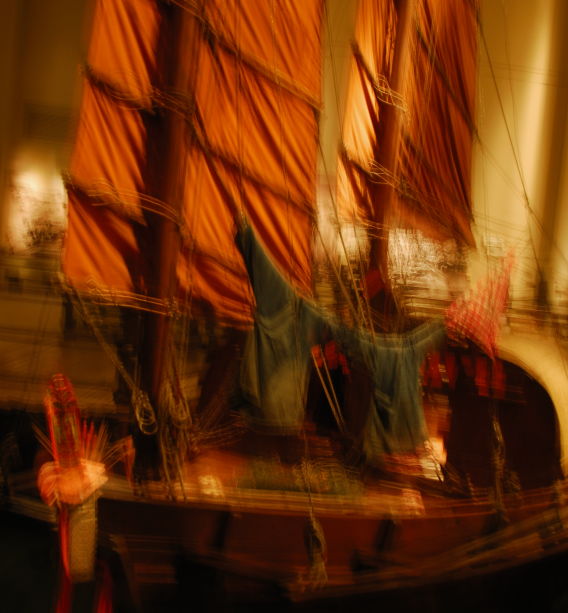
\includegraphics[width=0.3\textwidth]{DeblurOrig2.png}}
%%  \hspace{1em}
%  \subfigure[去模糊图像]{
%    \label{fig:deblur:e} %% label for second subfigure
%    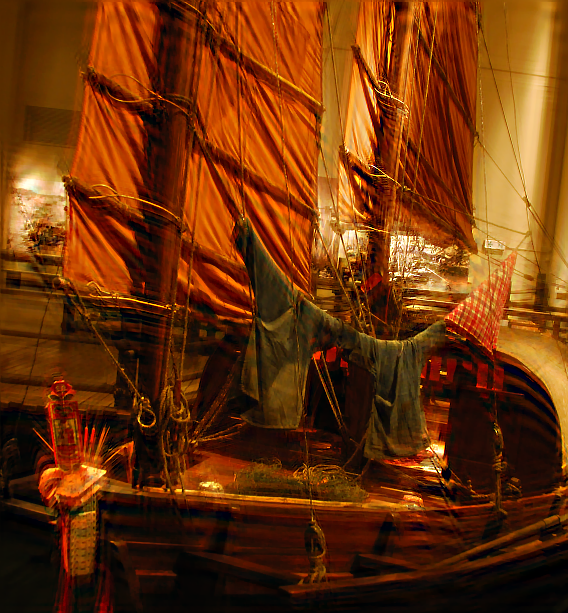
\includegraphics[width=0.3\textwidth]{DeblurResult2.png}}
  \caption{图像去模糊(Deblur)}
  \label{fig:deblur} %% label for entire figure
\end{figure}

\item \textbf{中文}:基于图像的参数回归。

\textbf{English}: Paramter Regression.

\textbf{简要说明}:图像中蕴含了成像介质的很多信息(参数),如何从图像中获取到这些信息是本研究方向的核心问题。此方向的研究思路比较新颖,并不能查到太多资料,如有问题请单独联系俞老师。

\textbf{主要方法}:深度神经网络(Deep Neural Network)
\end{enumerate}

\subsection{王楠}

\begin{enumerate}
\item 嵌入式编程及电路设计(机器人),此方向“软硬结合”,需要有单片机或电路设计经验。

\textbf{技能要求}:1)掌握C/C++编程,会进行图形化界面编程。2)对嵌入式系统有浓厚兴趣爱好,有ARM或FPGA开发经验者最佳。3)使用Altium Designer(DXP、Protel 99)等电路设计软件制作电路板。

在这里,你要做的事,\textcolor{red}{制作自己的机器人……当然,越智能越好。}
\item 数字图像处理,主要侧重模糊图像中目标边缘检测等。

\textbf{技能要求}:1)数学基础扎实。2)对“信号与系统”、“数字信号处理”有较好的领悟。3)掌握C/C++编程。

在这里,你要做的事,\textcolor{red}{结合机器人研发,探索如何在模糊不清的环境中进行目标检测,并进一步帮助机器人完成基于图像的路径规划等问题。}
\end{enumerate}

%%---------------------------------------------------------------------
\end{document}
